%!TEX root = internshipReport.tex

\chapter{BNP inference within PPLs} \label{BNP_PPL}
In this chapter we focus on the task of performing inference within a \gls{PPL} for models with an infinite dimensional component, also called \gls{BNP} models.
For now we have restricted ourselves to infinite mixture models, but we hope that our framework will enable efficient sampling for other \gls{BNP} models such as the infinite \acrlong{HMM} \cite{Beal02theinfinite}. We have also focused our study on \gls{MCMC} sampling methods, but \acrlong{VI} is considered in Section \ref{BNP_VI}. After introducing the ideas allowing to sample from \acrlongpl{PKP} prior, this section describes the methodology used for the experimentations, along with our contributions.

\section{Prior sampling for the \acrlong{DP}} \label{recursion}

In \glspl{PPL}, to transform a program variable \texttt{x} in a random variable, one only needed to write \texttt{x = sample(Dist(parameters))}. Then the posterior distribution (given some observations) of \texttt{x} will automatically be performed during the inference scheme.
The Bayesian setting thus naturally fits the framework of \glspl{PPL}.
Yet, we believe that there is more  than just a connection between Bayesian inference and \glspl{PPL}, but that there is also a connection between \acrlong{BNP} and High-order \gls{PPL}.

Working with \gls{BNP} models can be impossible because of the constraints of computers.
A \gls{NRM} $P$ can be written \cite{Kingman:1967kn} as
$$P = \sum_{k \ge 1}{{p}_k \delta_{X^\star_k}} \quad \text{and} \quad \sum_{k \ge 1}{p_k}=1$$
where $\left({p}_k, X^\star_k \right)_{k \ge 1}$ is an infinite collection of weights and atoms.
Discrete probability measures with countable support such as \acrlongpl{NRM} cannot be represented in a computer in a naïve manner since a machine has finite memory.
Other representations of such objects must be used, if one hope to denote them in a program.

One key notion in programming languages which will be crucial is the concept of \textit{lazy evaluation} (or \textit{laziness}). It is an evaluation strategy which delays the evaluation of an expression until its value is needed and which also avoids repeated evaluations.
Lazy evaluation is often combined with \textit{memoization}, as described in \cite{Bentley:1982:WEP:539147}. After a function's value is computed for that parameter or set of parameters, the result is stored in a lookup table that is indexed by the values of those parameters; the next time the function is called, the table is consulted to determine whether the result for that combination of parameter values is already available. If so, the stored result is simply returned. If not, the function is evaluated and another entry is added to the lookup table for reuse.

Instead of hoping to construct the entire infinite sequence $\left({p}_k, X^\star_k \right)_{k \ge 1}$, we will only ``lazily'' sample $\left({p}_k, X^\star_k \right)$, i.e. when we need them.
Since we work with homogeneous \glspl{CRM}, the $\{X^\star_k\}_{k \ge 1}$ are independent and identically distributed according to the base distribution. Sampling the $(X^\star_k)_{k \ge 1}$ as we need them is therefore trivial. Yet, how could we lazily sample the $({p}_k)_{k \ge 1}$ ?
In Subsection \ref{DP}, we presented the stick-breaking process, a generative process for constructing of a size-biased permutation of $({p}_k)_{k \ge 1}$, denoted $(\tilde{p}_k)_{k \ge 1}$.
In Section \ref{SBS} we explore other generative processes, for more generic \gls{BNP} classes. For now, Let us recall the construction given by \cite{sethuraman94} for the stick-breaking process of the \gls{DP}:


\begin{gather*}
V_k \stackrel{iid}{\sim} \text{Beta}(1, \alpha) \, \ k \ge 1 \\
\tilde{p}_k = V_k \prod_{j=1}^{k-1}(1-V_j)  \, \ k \ge 1
\end{gather*}

Therefore, $\tilde{p}_k$ can be seen as the probability of the following sequence of outcomes: $k-1$ Bernoulli draws with respective probabilities $V_j \ , j=1,\dots,k-1$, all yield failure, and one last Bernoulli draw with probability $V_k$ yields success.
How can this be interpreted as a generative process on an infinite set of discrete outcomes ?
%With this insight so as to sample from a \gls{CRP}, or equivalently from a \gls{DP} with a base distribution on the natural numbers.
Imagine ``walking'' down the natural numbers in order, flipping a coin with probability $V_k$ (called stick or stick length) for each one; if the coin comes up \texttt{false}, we continue to the next natural number; if the coin comes up \texttt{true}, we stop and return the current natural number. The probability of getting the natural number $k$ is given by $\tilde{p}_k$ defined above. This is formalised by the procedure \texttt{pickStick} in the code sample \ref{code:DP_SB} below. 

\begin{lstlisting}[caption={\acrlong{DP} stick-breaking representation written in Julia.},captionpos=b,label=code:DP_SB]
function pickStick(sticks, k)
  if rand(Bernoulli(sticks(k))) # flip a coin with weight $\tilde{p}_k$
    return k
  else
    return pickStick(sticks, k+1) # recursive call if coin is tail
  end
end

function DP($\alpha$)
  sticks = @memoize (index) -> rand(Beta(1, $\alpha$))
  return pickStick(sticks, 1)
end
\end{lstlisting}

The individual $V_k$ are drawn lazily, only generating new ones when we have walked out further than the furthest previous time. This is the role of the procedure \texttt{DP} which uses memoization to enforce this property. Even though we started by imagining an infinite set of sticks we only ever construct a finite subset of them. The above generative construction of the \gls{DP} defines a distribution over the infinite set of natural numbers, which is equivalent to the \gls{CRP} defined in Section \ref{DP}.

Note that the function \texttt{pickStick} is written in a special fashion: it is built via a \textit{recursion}. A \textit{recursive} function has one or more base cases for which the function produces a result trivially (without recurring), and one or more recursive cases for which the program recurs (calls itself). For programming languages, allowing recursion means allowing a function to call itself within the program text. Moreover, before calling \texttt{pickStick}, the program does not know the integer which will be returned, i.e. the number of recursion calls, since it is a random variable by construction.

Recall that high-order \glspl{PPL} allow complex control flow, including stochastic recursion (stated in Section \ref{PPL_history}). \textit{Stochastic} or \textit{unbounded} recursion simply means that the number of recursive calls (also called \textit{depth} of the recursion) is random or unbounded. Therefore, the \gls{DP} stick-breaking process can be written and executed with such high-order \glspl{PPL}.

\glspl{PPL} are some sort of \textit{simulators}, models need to be written as generative processes. Executing such a model -- as is -- via a \gls{PPL}'s interpreter, is sampling from its prior distribution. Once one can write a model as a generative process, (i.e can sample from the model's prior), the \gls{PPL} can perform inference on the latent variables. Consequently, for \gls{BNP} models based on \acrlongpl{RPM}, a representation similar to the stick-breaking process for the \gls{DP}, seems to be necessary.

\subsection{From sampling in $\mathbb{N}$ to sampling in $\Omega$}
The stick-breaking construction previously described defines a distribution over the infinite set of natural numbers via the sequence of weights $(\tilde{p}_k)_{k \ge 1}$, as the \gls{CRP} does. Yet, ultimately we would like a distribution not over the natural numbers themselves, but over an infinite set of samples from some other distribution $H_0$ (called the base distribution) which will represent our mixture components. Using the homogeneous assumption (of the underlying \gls{CRM}), we can easily generalise the \gls{DP} code that we wrote to this setting by using \texttt{@memoize} to associate to each natural number, a draw from the base distribution.
This is what the code sample (\ref{code:DP}) below formalises.

\begin{lstlisting}[caption={\acrlong{DP} with base distribution $H_0$ written in Julia.},captionpos=b,label=code:DP]
function DPmem($\alpha$,$H_0$)
  augmentedDP = @memoize (stickIndex) -> rand($H_0$)
  return () -> augmentedDP(DP($\alpha$)) # returns a lambda function
end
\end{lstlisting}

\subsection{Stochastic memoization}
Discrete Random Probability Measures can be seen through the interesting perspective of \textit{stochastic memoization} \footnote{\url{https://probmods.org/chapters/12-non-parametric-models.html}}, which is an in-between (deterministic) memoization and no memoization.
Higher-order procedures such as \texttt{DPmem} (defined above) transform a procedure into one that sometimes reuses its returned values, and sometimes generate new values. These procedures are called \textit{stochastic memoizers} by Goodman et al. \cite{Goodman:2012uq}.
For instance with the \gls{DP}, setting $\alpha = 0$ recovers a deterministic memoization whereas setting $\alpha \rightarrow \infty$ yields no memoization at all.

\subsection{Prior sampling algorithm}
We have implemented in Listing \ref{code:DP_SB} the stick-breaking construction with a recursive function. Yet, this is not the most efficient implementation of such a generative process. Consider that the concentration $\alpha$ is quite big, then the sticks $V_k \sim \text{Beta}(1, \alpha)$ will tend to be small. Consequently, calling \texttt{DP} (thus \texttt{pickStick(sticks, 1)}) will tend to flip many coins before one yields head (way more than the number of atoms already sampled). Having to go through lots of these sticks, for each point that is sampled from the \gls{DP} sample can be computationally intensive.

Since $\sum_{k=1}^\infty{p_k} = 1$, the \gls{DP} can be seen as an infinite categorical distribution. Yet, it can be lazily cast as a finite categorical distribution with $k+1$ categories, after having sampled $k$ atoms; the $k$ existing atoms and one other category corresponding to a non-sampled yet atom. The weights of such a finite categorical distribution are $(\tilde{p}_1, \dots, \tilde{p}_k, 1-\sum_{k=1}^\infty{\tilde{p}_k})$. Such weights can easily be computed since $V_k \sim \text{Beta}(1, \alpha)$ and $\tilde{p}_k = V_k  (1-\sum_{j=1}^{k-1}{\tilde{p}_j})$.

We have empirically assessed the computation needs of these two implementation by sampling $10000$ different \glspl{DP}, and then sampling $1000$ points from each of them. Results have been summed up in Figure \ref{fig:prior_sampling_perf}. By using a recursive sampling, it appears that the computation time grows linearly with $\alpha$, whereas it is constant by using the previously described algorithm.

\begin{figure}[h!]
\centering
    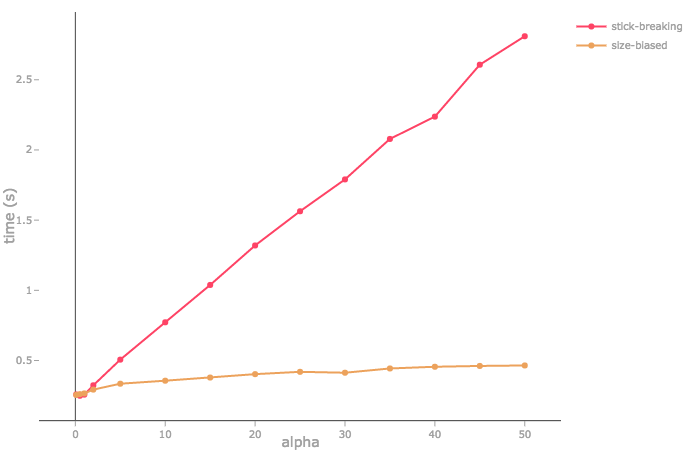
\includegraphics[width=0.7\linewidth]{prior_sampling_perf.png} 
    \caption{Computational time to sample $1000$ points from a \gls{DP}, averaged on $10000$ runs.}
    \label{fig:prior_sampling_perf} 
\end{figure}

Even if the stochastic recursion perspective is an elegant one, the categorical sampling algorithm is a better way to sample from a \gls{DP} from a computational point of view.

% \subsection{Implementation details}
% As highlighted, recursion is key to denote \gls{BNP} models in a \gls{PPL}.
% A function is called \textit{tail-recursive} when the recursive call happens as the final action in a function (as for \texttt{pickStick}), in which case it can happen without the function call stack growing. In \gls{CPS}, there is no stack -- all function calls are tail calls, hence all recursive functions are tail-recursive.

% Clojure provides special forms \emph{loop} and \emph{recur} for writing tail-recursive programs. Anglican programs are \gls{CPS}-converted and do not use the stack. Therefore recursive calls in the Anglican \gls{PPL} cannot lead to stack overflow.
% Without such a specific \emph{recur} operator, the call stack can exceed its maximum size and yields errors.

\subsection{Existing work}

Most high-order \glspl{PPL} indeed already handle some \gls{BNP} models \cite{Goodman:2012uq,wood-aistats-2014,probmods2}.
See \footnote{\url{http://www.robots.ox.ac.uk/~fwood/anglican/examples/index.html}} for Anglican's examples of Hierarchical Dirichlet Process or Probabilistic Deterministic Infinite Automata. See also \footnote{\url{https://probmods.org/chapters/12-non-parametric-models.html}} for WebPPL's example of Infinite Hidden Markov Models or Infinite Relational Model.
Yet, their experimentations are mostly limited to \acrlong{DP}, \acrlong{PY} or hierarchical versions of these processes, and often focused on sampling from priors. When performing inference,
the used scheme is usually a particle algorithm such as \acrlong{SMC} or \acrlong{CSMC}.


\section{Generative constructions of random probability measures} \label{SBS}
Previously, we recalled that to be able to denote a model in a \gls{PPL}, one should know how to sample from its prior, i.e. know a generative construction.
% We also highlighted the fact that such generative processes can be implemented via stochastic recursion.

\subsection{Stick-breaking processes} \label{stick-breaking}

The first comprehensive treatment of stick-breaking priors dates back to the paper by Ishwaran and James \cite{Ishwaran:2001dw}. There, they introduced a class of stick-breaking priors including as special cases the \acrlong{DP} by Ferguson \cite{ferguson73} and the two parameter Poisson-Dirichlet process by Perman et al. \cite{Perman:1992ke}. Specifically, let $H_0$ be a nonatomic probability measure on a complete and separable metric space $\mathbb{X}$.
% equipped with the Borel σ-field X .
Also, let $(V_i)_{i \ge 1}$ be a sequence of independent random variables such that $\sum_{i \ge 1}{\mathbb{E}[\log(1 - V_i)]} = - \infty$.
Based on such $V_i$'s, they define a sequence of random probabilities $(\tilde{p}_k)_{k \ge 1}$ as $\tilde{p}_1 = V_1$ and
\begin{equation} \label{eq:Stick_breaking}
\tilde{p}_k = V_k \prod_{j=1}^{k-1}{(1-V_j)} 
\end{equation}
for each $k > 1$, and let $(X^\star_k)_{k \ge 1}$ be a sequence of random variables, independent
of $(\tilde{p}_k)_{k \ge 1}$, and independent and identically distributed according to $H_0$. Then,
$$ P = \sum_{k \ge 1}{\tilde{p}_k \delta_{X_k^\star}} $$
is a stick-breaking prior in the class of Ishwaran and James \cite{Ishwaran:2001dw}.

For any $\sigma \in [0,1)$ and $\theta > -\sigma$, the stick-breaking representation of the two parameter Poisson-Dirichlet process is recovered by assuming the $V_k$'s to be distributed according to the Beta distribution with parameter $(1 - \sigma, \theta + k\sigma)$ for each $k \ge 1$.
The stick-breaking representation of the \gls{DP}, which was first derived by Sethuraman \cite{sethuraman94}, is also recovered as special case, by setting $\sigma = 0$.

Apart from the two parameter Poisson-Dirichlet process, most of the discrete random probability measures do not admit a stick-breaking representation in terms of a collection of independent $V_i$'s.%, but in terms of conditional distributions of $Z_k$'s given $(Z_1,\dots,Z_{k-1})$.

As an example, Favaro et al. \cite{Favaro:2012ht} derived the stick-breaking representation of the normalized inverse Gaussian process introduced in Lijoi et al. \cite{Lijoi:2005ku}. Specifically, let $b > 0$ and let $(V_k)_{k \ge 1}$ be a sequence of dependent random variables such that, for each $k \ge 1$, the conditional distribution of $V_k$ given $(V_1,\dots,V_{k-1})$ coincides with the distribution of the random variable
\begin{equation} \label{eq:IGP}
\frac{X_k}{X_k + Y_k}
\end{equation}
where $X_k$ is distributed according to the generalized inverse Gaussian distribution and $Y_k$ is distributed according to the positive $\frac{1}{2}$-stable distribution.

According to Favaro et al \cite{Favaro:2014bo}, the normalized inverse Gaussian process \cite{Favaro:2012ht} is the first example of a prior admitting a stick-breaking representation in terms of dependent  $V_k$'s, and such that for any $k \ge 1$ the conditional distribution of $V_k$ given $(V_1,\dots,V_{k-1})$ is characterized by means of a straightforward transformation of random variables as in \ref{eq:IGP}.
Favaro et al \cite{Favaro:2014bo} construct a similar transformation to build a stick-breaking process for a subclass of $\sigma$-stable Poisson-Kingman processes.
Similarly, James \cite{James:2013uk} builds a stick-breaking process for the class of $\text{PG}(\alpha,\zeta)$-Generalized Gamma Processes.
% The $V_k$'s can be generated via the following construction:
% \begin{gather*}
% \zeta_0 \sim \zeta \\
% \vdots \\
% \zeta_k = \zeta_0 + \sum_{j=1}^{k-1}{e_j},\ e_j \sim \text{Exp}(1) \\
% R_k = \left(\frac{\zeta_{k-1}}{\zeta_k}\right)^{1/\alpha} \\
% V_k = 1 - \beta_k(1 - R_k), \ \beta_k \sim \text{Beta}(1-\alpha,\alpha) \\
% \vdots \\
% \tilde{p}_k = V_k \prod_{j=1}^{k-1}(1-V_j) \ \ ,k= 1,2,\dots
% \end{gather*}

Since the size-biased sequence of weights $(\tilde{p}_k)_{k \ge 1}$ is defined through Equation \ref{eq:Stick_breaking} for stick-breaking processes, it can be generated in the same way as described in the previous Section \ref{recursion}: drawing Bernoulli's with parameters $V_k$'s until success, then return integer $k$.
% Stochastic recursion is therefore the crux of the  implementation of stick-breaking processes in \glspl{PPL}.

\subsection{Size-biased generative processes}
% \subsection{\acrlong{PKP}}

The \gls{PKP} generative process (\acrlong{SBS}) described in Section \ref{PKP}, is reminiscent of the well known stick breaking construction from Ishwaran \& James \cite{Ishwaran:2001dw}, where a stick of length one is successively broken as in Figure \ref{fig:PY_stick_breaking}.
This \gls{SBS} process is illustrated in Figure \ref{fig:PK_generative_process} and schematically recalled below:
\begin{gather*}
T \sim \gamma \\
\tilde{J}_1|T \sim \text{SBS}(T) \\
\tilde{J}_2|T,\tilde{J}_1 \sim \text{SBS}(T - \tilde{J}_1) \\
\vdots \\
\tilde{J}_{l}|T,\tilde{J}_1,\dots,\tilde{J}_{l-1} \sim \text{SBS}(T - \sum_{i<l} \tilde{J}_i) \\
\vdots \\
\end{gather*}
\begin{figure}[h!]
  \centering
  \begin{minipage}[b]{0.48\textwidth}
    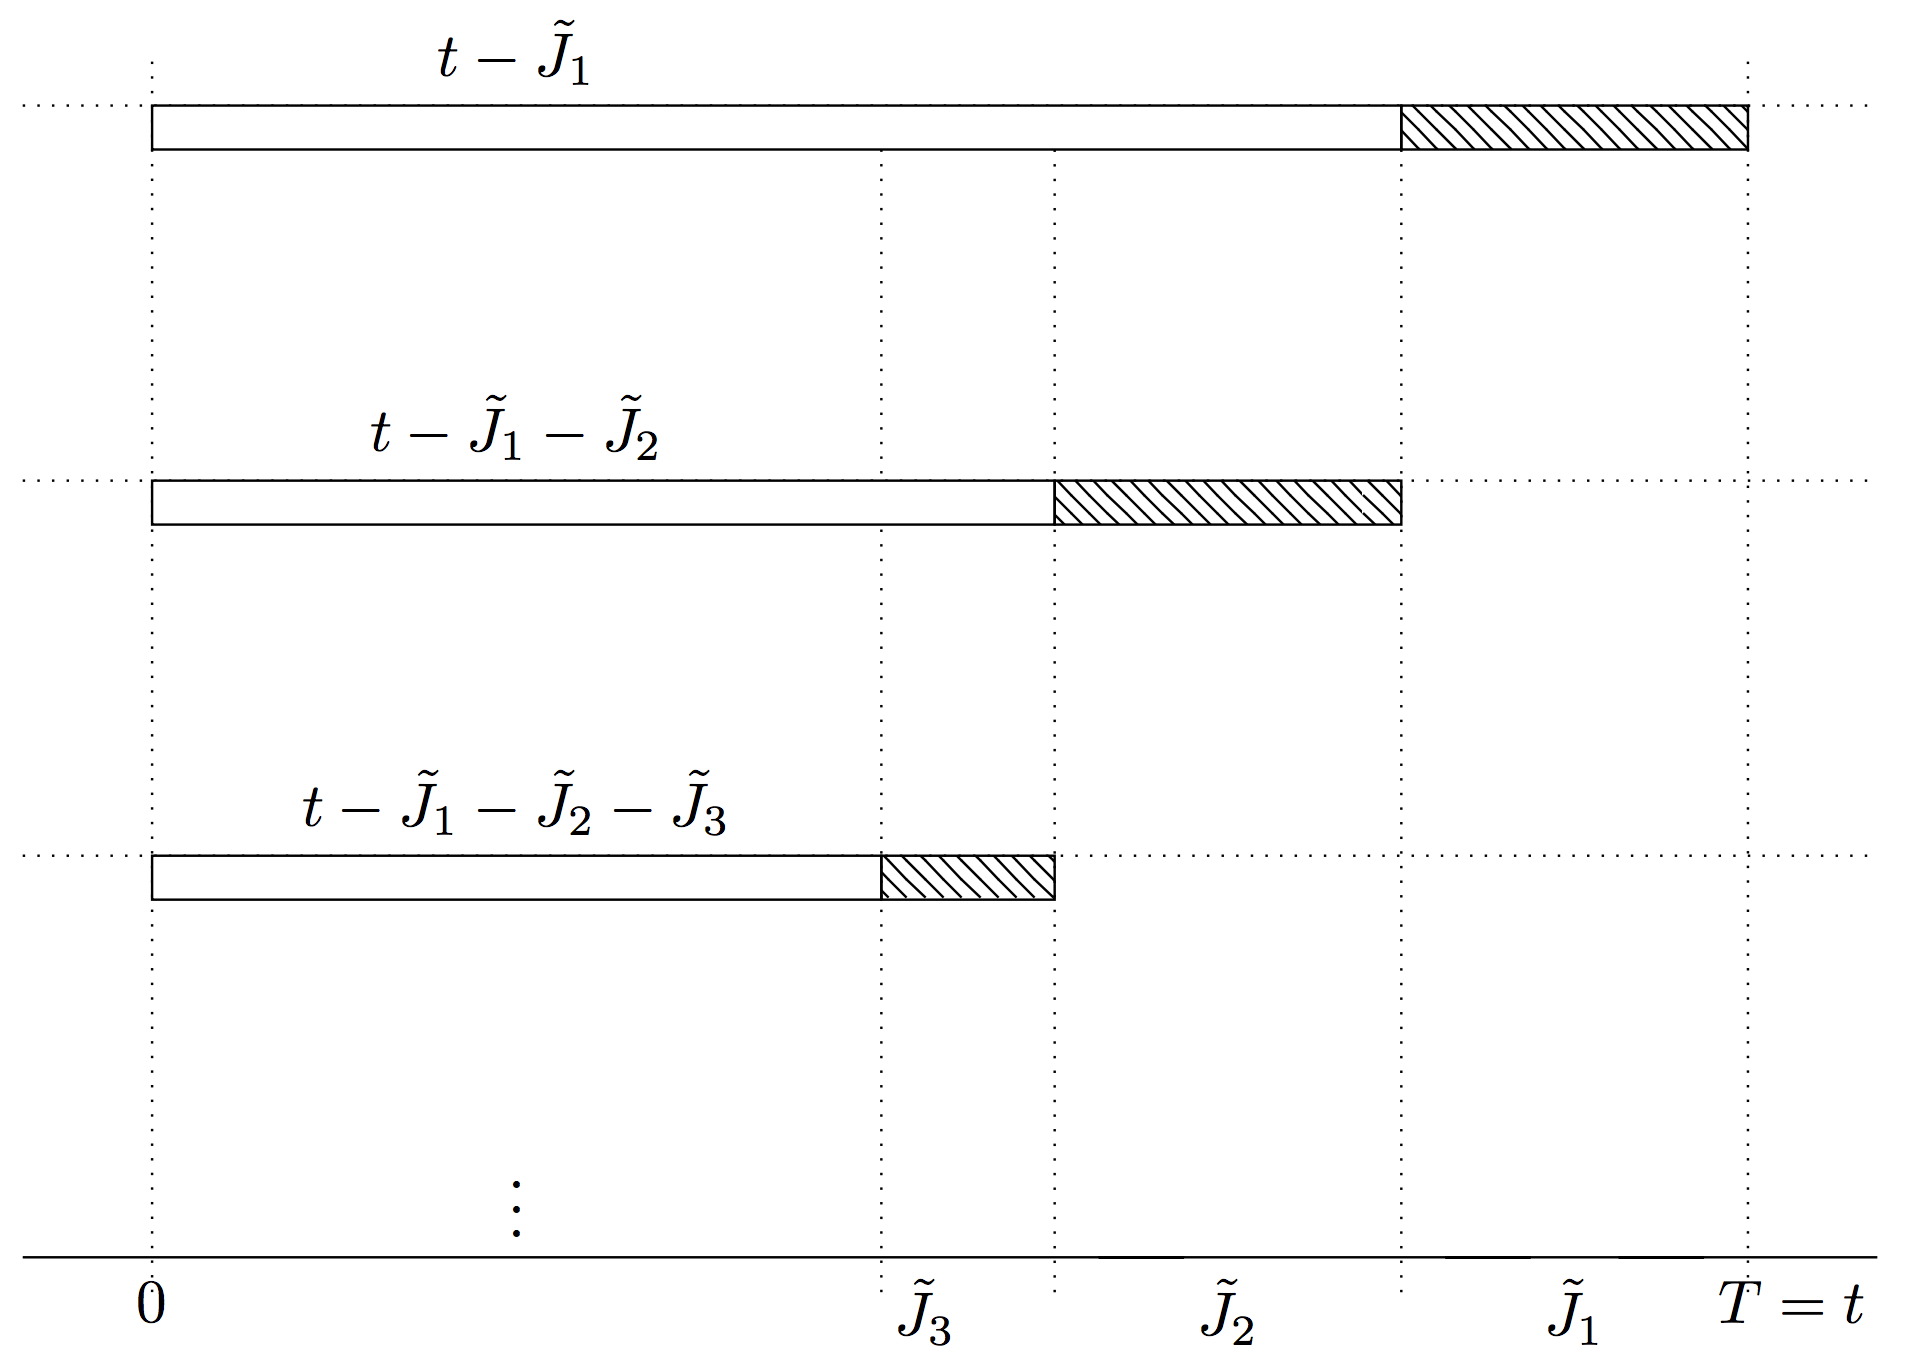
\includegraphics[width=\textwidth]{PK_generative_process2.png}
    \caption{Generative process of Poisson-Kingman Process. Source: \cite{LomeliThesis}.}
    \label{fig:PK_generative_process}
  \end{minipage}
  \hfill
  \begin{minipage}[b]{0.48\textwidth}
    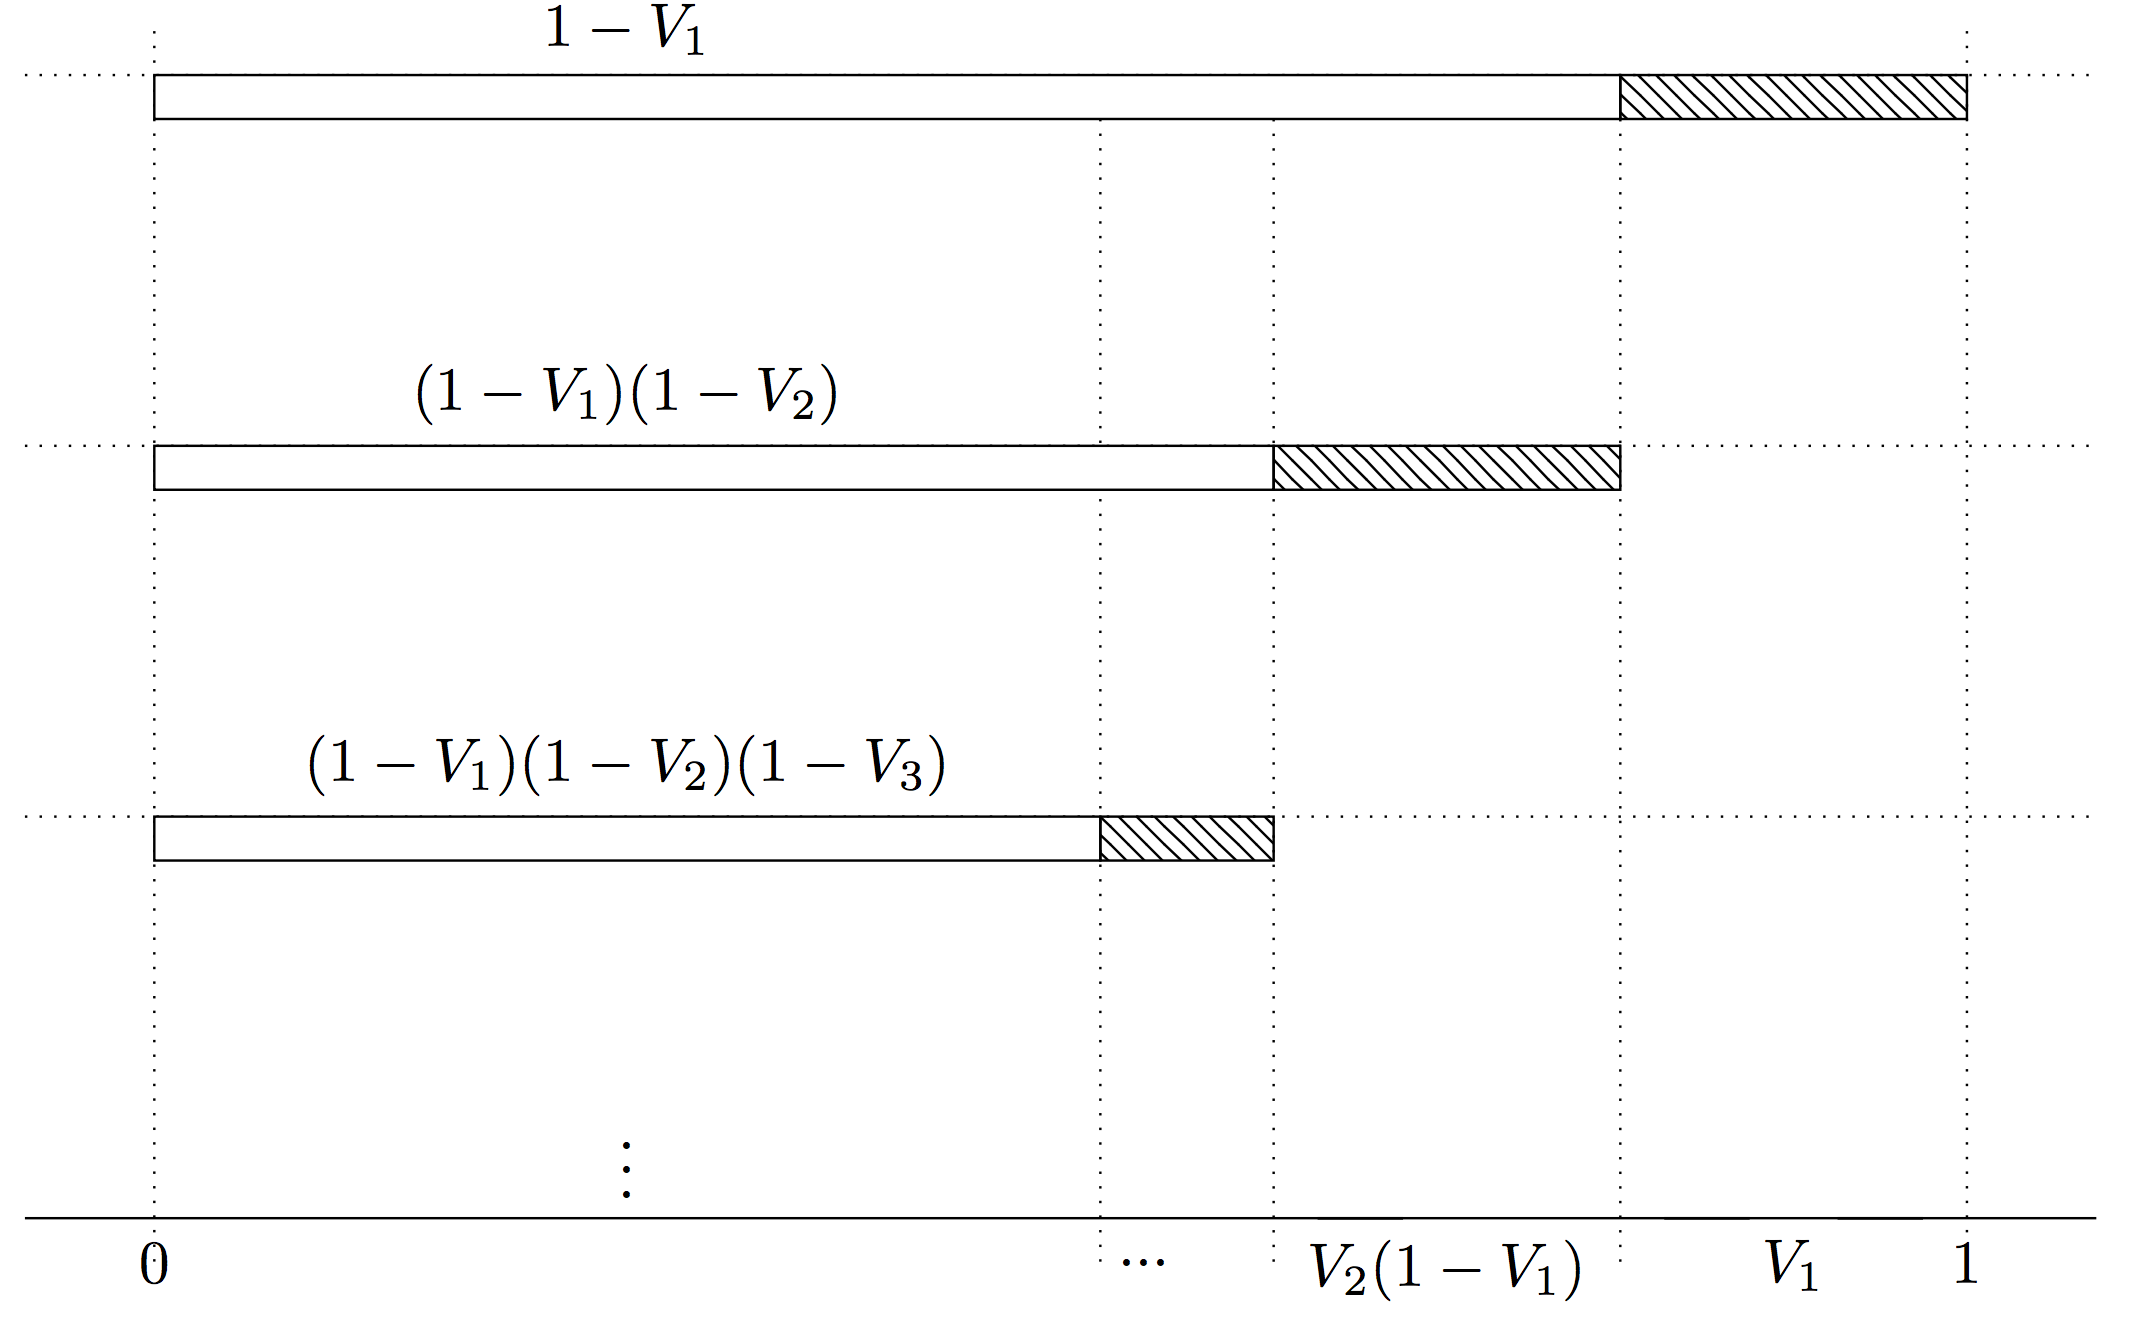
\includegraphics[width=\textwidth]{PY_stick_breaking2.png}
    \caption{Stick-breaking construction. Source: \cite{LomeliThesis}.}
    \label{fig:PY_stick_breaking}
  \end{minipage}
\end{figure}
However, by starting with Equation (\ref{eq:perman2}), one can recover the usual stick-breaking construction due to two useful identities (in distribution):
\begin{equation} \label{eq:SBS1}
\tilde{p}_k := \frac{\tilde{J}_k}{T} \ \text{for} \ k=1,\dots
\end{equation}
\begin{equation} \label{eq:SBS2}
V_k := \frac{\tilde{p}_k}{1 - \sum_{j=1}^{k-1}{\tilde{p}_j}} \ \text{for} \ k=1,\dots
\end{equation}

Indeed, equivalently to Equation (\ref{eq:SBS2}), we have $\tilde{p}_k = V_k \prod_{j=1}^{k-1}{(1-V_j)}$ for all $k \ge 1$, which is of the same form as Equation (\ref{eq:Stick_breaking}) for the usual stick-breaking process.
In general, the stick random variables $(V_k)_{k \ge 1}$ from Equation (\ref{eq:SBS1}), form a sequence of dependent random variables, except for some simple processes as the \gls{DP} and \gls{PY}, see Pitman \cite{PitmanRDD} for details.
Similarly to stick-breaking constructions, \acrlongpl{PKP} can therefore be constructed in a generative manner and implemented via (stochastic) recursion.

%(\ref{eq:perman2})
%By reparameterizing the model using these identities and then obtain the corresponding joint in terms of $(0,1)$-valued stick-breaking weights $\{{V}_k\}_{k \ge 1}$ which correspond to the usual stick-breaking representation. This joint distribution is for a general Lévy measure $\rho$, density $f_\rho$ and it is conditioned on the valued of the random variable $T$.
%The standard Stick breaking representations can be recovered for the Dirichlet and Pitman-Yor processes, for a specific choice of $\rho$ and if we integrate out T. For instance, the \gls{PY} stick breaking representation \cite{Ishwaran:2001dw} can be recovered from the \acrlong{SBS} generative process of Section 2.5 after integrating out the total mass $T$, a change of variables and the following distribution for the total mass is substituted
%$$ \gamma_{\text{PY}}(t) = \frac{\Gamma(\theta+1)}{\Gamma(\theta / \alpha + 1)}t^{-\theta} f_\sigma(t) 1_{(0,\infty)}(t), \quad \theta > -\sigma $$
%where $f_\sigma$ is the density of a $\sigma$-Stable random variable.

\paragraph{Practical aspects of \gls{SBS}}

A useful identity for computing sticks length $(V_k)_{k \ge 1}$ is given by
\begin{equation} \label{eq:SBS4}
V_k = \frac{\tilde{J}_k}{T_{k-1}} \quad \text{for} \ k=1,\dots
\end{equation}
Consequently, to compute $V_k$, one only needed to sample $\tilde{J}_{k}|T,\tilde{J}_1,\dots,\tilde{J}_{k-1}$, and to update the surplus mass given by $T_1 = T$ and $T_k = T - \tilde{J}_k$ for $k \ge 2$.
The normalised weights $(\tilde{p}_k)_{k \ge 1}$ are therefore never computed.

In the \acrlong{SBS} process (described in Section \ref{PKP}), when a random variable $X_i$ takes the value of an atom which has not yet been sampled, a new atom $X^\star_{k+1}$ must be sampled, along with its associated weight $\tilde{J}_{k+1}$. The new atom $X_{k+1}^\star$ is drawn from $H_0$, while its associated normalised weight is drawn from
\begin{equation} \label{eq:SBS3}
\mathbb{P}_{\rho,H_0}(\tilde{J}_{k+1} \in ds_{k+1} | T \in dt_k) = \frac{s_{k+1}}{t_k}\rho(ds_{k+1})\frac{f_\rho(t_k - s_{k+1})}{f_\rho(t_k)}
\end{equation}

Yet, even if we know the density of the distribution of $\tilde{J}_{k}|T,\tilde{J}_1,\dots,\tilde{J}_{k-1}$, we do not necessarily know how to sample from it.
We are currently working on a generic way to sample from such as distribution. We could restrict to Lévy measures with tractable intensity -- which can be evaluated pointwise -- thus excluding $\sigma$-Stable \gls{PK}. A simple rejection sampling scheme with proposal $\mathcal{U}(0, T_k)$ might be sufficient.
Nonetheless, there are particular cases for which we already know how to sample from these distributions. Lomeli et al \cite{Lomeli:2015vd} proposes a simple rejection sampling scheme with uniform proposal to tackle the $-\log$Beta \gls{PK} process. Favaro et al \cite{Favaro:2014bo} gave an identity from which iid samples can be drawn for a subclass of $\sigma$-Stable \gls{PKP}.

One of our contribution is the implementation of building blocks to sample from \acrlongpl{NRM} and \acrlongpl{PKP}. The code can be found online \footnote{\url{https://github.com/emilemathieu/Turing.jl/tree/feature-328/src/models}}. The only function which needs to be implemented to be able to sample from a specific class of \acrlong{RPM} is \texttt{sampleWeight} which samples $\tilde{J}_{k+1}$ given $\{T,\tilde{J}_{1},\dots,\tilde{J}_{k}\}$. We have specifically implemented this for the \gls{DP} and the $-\log$Beta \gls{PK} process. See for instance samples from a $-\log$Beta \gls{PK} process in Figure \ref{fig:logBetaPK}.

\begin{figure}[h!]
\centering
    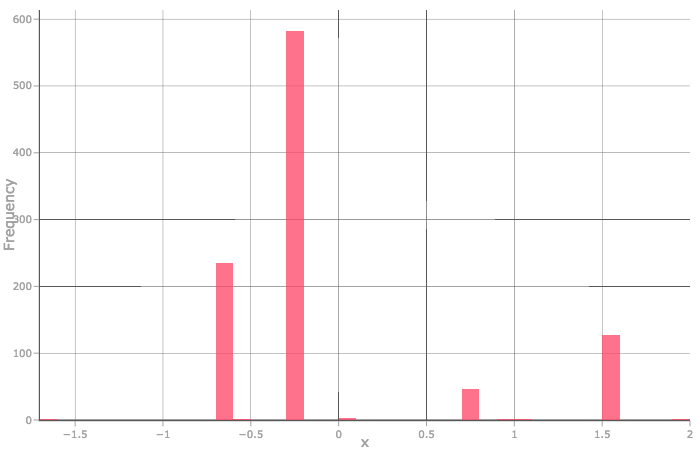
\includegraphics[width=0.7\linewidth]{logBetaPKRandomMeasure.png} 
    \caption{Histogram of $1000$ samples from a $-\log \text{Beta}(1,2)$ \acrlong{PK} random measure.}
    \label{fig:logBetaPK} 
\end{figure}

\section{Models of interest}
We focus on infinite mixture models described in Section \ref{mixture_models}.
We use a \acrlong{DP} as a prior over mixture components so as to build an infinite Gaussian mixture model.
Yet, the \gls{DP} could be replaced by another \acrlong{NRM} or \acrlong{PK}.

More specifically we consider for our experimentations the following hierarchical model
\begin{gather*}
\theta \sim \text{InverseGamma}(\alpha_0, \beta_0) \\
P \sim \text{DP}(\alpha, \mathcal{N}(m_0, \sqrt{v_0})), \\
X_i|P \sim P, \\
Y_i|X_i \sim \mathcal{N}(X_i, \sqrt{\theta}) \\
\end{gather*}

The equivalent model written in Turing can be found in the code sample \ref{code:IMM} below.
The real code of the size-biased processes and the infinite mixture model which has been used for our experimentations can be found on Github \footnote{\url{https://github.com/emilemathieu/Turing.jl/tree/feature-328/src/models}}.

\begin{lstlisting}[caption={Nonconjugate infinite mixture model written in Turing.jl.},captionpos=b,label=code:IMM]
@model InfiniteMixutre(y) = begin
  N = length(y)
  $\alpha$ =  10.0
  $\theta$ ~ InvGamma(precisionShape, precisionScale) # Sample statement
  P ~ DP($\alpha$, Normal(meanMean, meanStd)) # Sample statement

  x = zeros(N)
  for i in 1:N
    x[i] ~ P # Sample statement
    y[i] ~ Normal(x[i], sqrt($\theta$)) # Observe statement
  end
end
\end{lstlisting}

This model is a Gaussian mixture model with a shared variance of all clusters according to line \texttt{10}. This variance is distributed according an inverse gamma distribution as specified in line \texttt{4}.
The base measure of the \gls{DP} is a normal distribution as shown in line \texttt{5}.

Turing uses an unique symbol \texttt{$\sim$} to denote sampling and observation. This model (function) is then compiled to replaced this symbol by the appropriate function: \texttt{sample} or \texttt{observe}. If the left-hand side term of \texttt{$\sim$} is unknown, it is a random variable and \texttt{sample} is consequently chosen. Otherwise, if the term is a deterministic value (such as \texttt{y[i]}s), \texttt{observe} is chosen. This is written in the comments of the above code sample \ref{code:IMM} after symbols \texttt{\#}.

\section{Posterior samplers} \label{sec:posterior_sampler}

Now that we have described and implemented a way to sample from the (prior) distribution of an infinite mixture model, we focus on the issue of sampling from the posterior distribution $ p(\theta, x_{1:T}|y_{1:T}) \propto p(\theta, x_{1:T},y_{1:T})$. In Chapter 5 on \acrlongpl{PPL}, we presented many different inference schemes. These schemes are generic, meaning that for any model, they will produce samples that are distributed according to the targeted posterior distribution. Yet, this assertion does not give any guaranty on the quality of the produced samples.

Indeed, \glspl{PPL} makes a trade-off between flexibility and efficiency. In an high-order \gls{PPL} where a huge class of models can be represented, it is hard to develop inference schemes which are efficient for all possible models. Whereas for a first-order \gls{PPL} as Stan which can only represent finite dimensional graphical models, developing an efficient inference scheme is easier since the denotable class of models is relatively small.
By \textit{efficient}, we mean for a sampler to be able to produce samples with "high" \textit{quality} for some given computational resources. The quality is usually defined in term of \acrfull{ESS} \footnote{\url{https://en.wikipedia.org/wiki/Effective_sample_size}} which is a measure of correlation between produced samples.
The spirit of \glspl{PPL} from our belief is then to have multiple inference schemes, which could be combined, such that these schemes are efficient on different subclasses of representable models.

The goal of this internship has therefore been to find or develop an efficient algorithm to produce samples distributed according to the posterior distribution of the previously described infinite mixture model.

\subsection{\acrlong{SMC}}
By writing the infinite mixture model as in Listing \ref{code:IMM} above -- using the \texttt{for-loop} form -- the model is expressed as a \acrlong{SSM}. Such a formulation allows to make use of particle algorithms (see Subsections \ref{IS} and \ref{PMCMC}) thanks to the sequence of \texttt{observe} statements.

As described in Section \ref{IS}, the \acrfull{SMC} algorithm breaks down the overall inference problem into a series of target distributions which get incrementally closer to the distribution of interest. These intermediate target distributions live in smaller spaces than the overall posterior distribution. This class of methods is consequently well suited as a generic inference method for the high-dimensional models that we are considering. It is straightforward to prove that by using an \gls{SMC} scheme within a \gls{PPL} with our model, we are indeed rightly targeting the posterior distribution.

\subsection{\acrlong{PG}}
By using \gls{SMC}, the random global parameter $\theta$ (precision of the Gaussian mixtures) would also be included in the latent space and sampled at the same time as the mixture components and assignments. More precisely, it would be re-sampled with all hidden (non-observed) variables appearing before the first \texttt{observe statement}; therefore with $x_1$ (\texttt{x[1]} at line \texttt{9}).
If the mixing of the posterior samples of $x_1$ (and consequently of $\theta$) is poor, it would negatively affect the mixing of the $(x_2,\dots,x_T)$ samples.

\acrlong{PMCMC} methods -- introduced by Andrieu et al \cite{Andrieu:2010gc} -- alleviate this issue by explicitly targeting $ p(\theta, x_{1:T}|y_{1:T}) \propto p(\theta, x_{1:T},y_{1:T})$, thus decoupling the global parameters $\theta$ from the (states) $x_{1:T}$.
These algorithms -- such as \acrlong{PG} and \acrlong{PMMH} -- use \gls{SMC} algorithms to design efficient high dimensional proposal distributions for \gls{MCMC} algorithms.

As already described in Section \ref{PMCMC}, the \gls{PG} algorithm is a Gibbs sampler which iteratively samples from $p(\theta|x_{1:T},y_{1:T})$ and $p_\theta(x_{1:T}|y_{1:T})$, with $x_{1:T} \sim p_\theta(\cdot|y_{1:T})$ being generated by a Conditional \gls{SMC} update. This update is similar to a standard \gls{SMC} algorithm but is such that a prespecified path $x^\star_{1:T}$ (the previously generated value $x_{1:T}$ in the Gibbs step) is ensured to survive all the resampling steps, whereas the remaining $N-1$ particles are generated as usual.

% This is obviously inefficient and \acrlong{PMCMC} methods should perform better for this random parameters setting.


We therefore experimented using \acrlong{PG} targeting the cluster components and assignments $x_{1:T}$ with the conditional \gls{SMC} and the global parameter $\theta$ with an \gls{HMC}. The \gls{PG} algorithm was already implemented in Turing, so there is no contribution from us for the \gls{PG} algorithm.
All our experimentations are using the galaxy data set 
\footnote{Consists of the following values: 9172,9350,9483,9558,9775,10227,10406,16084,16170,18419,18552,18600,\\18927,19052,19070,19330,19343,19349,19440,19473,19529,19541,19547,19663,19846,19856,19863,19914,19918,\\
19973,19989,20166,20175,20179,20196,20215,20221,20415,20629,20795,20821,20846,20875,20986,21137,21492,\\
21701,21814,21921,21960,22185,22209,22242,22249,22314,22374,22495,22746,22747,22888,22914,23206,23241,\\
23263,23484,23538,23542,23666,23706,23711,24129,24285,24289,24366,24717,24990,25633,26960,26995,32065,\\
32789,34279.} 
as observations, which consists of the velocities at which 82 galaxies are receding away from our own. We are using Turing for our experimentations.
Figure \ref{fig:posterior_samples_time} shows 100 samples from the posterior distributions of mixture components $X_1$ and $X_{82}$. These samples have been generated from a \gls{PG} with 50 particles. The \gls{ESS} is computed on 50 samples for each $t$, and these \glspl{ESS} are then averaged on 8 runs. One can note from Figure \ref{fig:posterior_samples_time} that samples from $X_1$ are very ``sticky'', compared to samples from  $X_{82}$. Figure \ref{fig:ess} highlights this phenomenon, since we can see that the first $X_t$'s drastically have lower \gls{ESS} (meaning poorer mixing) than the $X_t$'s at the end of the sequence ($t$ close to 82). 


\begin{figure}[h!]
\centering
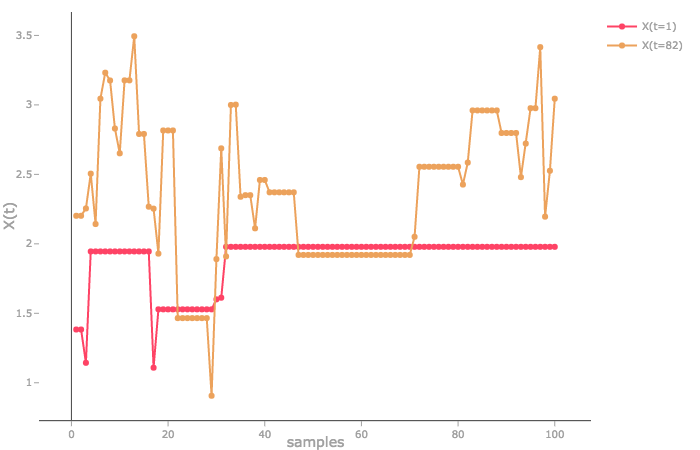
\includegraphics[width=0.8\textwidth]{samples.png}
    \caption{Samples from the Particle Gibbs sampler (with 50 particles) for the first ($t=1$) and the last ($t=82$) mixture components.}
    \label{fig:posterior_samples_time}
\end{figure}


\begin{figure}[h!]
\centering
    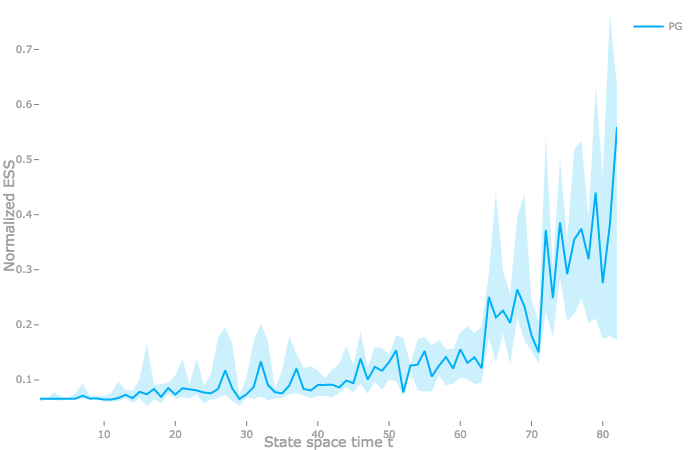
\includegraphics[width=0.8\textwidth]{ESS_PG_1.png}
    \caption{Normalized \acrfull{ESS} for 50 samples generated via Particle Gibbs with 50 particles. This \gls{ESS} is averaged on 8 runs.}
    \label{fig:ess}
\end{figure}


% \begin{figure}[h!]
%   \centering
%   \begin{minipage}[b]{0.48\textwidth}
%     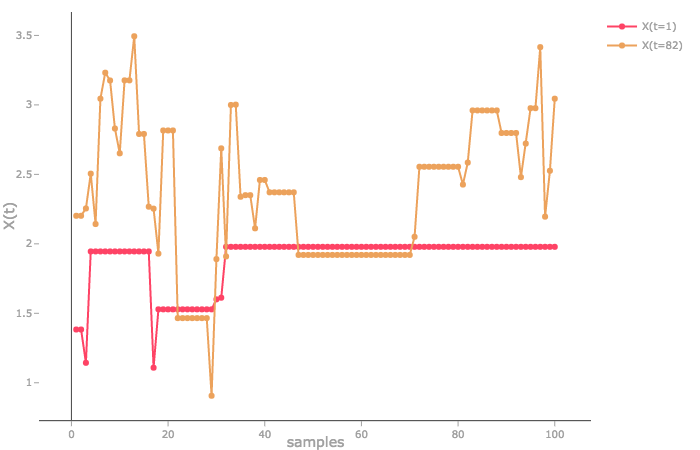
\includegraphics[width=\textwidth]{samples.png}
%     \caption{Samples from the Particle Gibbs sampler (with 50 particles) for the first ($t=1$) and the last ($t=82$) mixture components.}
%     \label{fig:posterior_samples_time}
%   \end{minipage}
%   \hfill
%   \begin{minipage}[b]{0.48\textwidth}
%     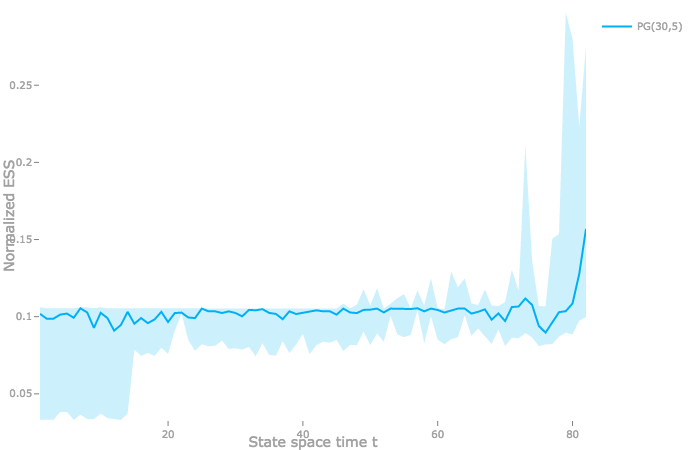
\includegraphics[width=\textwidth]{ESS3.png}
%     \caption{Normalized \acrfull{ESS} for 30 samples generated via Particle Gibbs with 5 particles. This \gls{ESS} is averaged on 10 runs.}
%     \label{fig:ess}
%   \end{minipage}
% \end{figure}

Indeed, a drawback of \gls{PG} is that it can be particularly adversely affected by \textit{path degeneracy} in the \gls{CSMC} step. Conditioning on an existing trajectory means that whenever resampling of the trajectories results in a common ancestor, this ancestor must correspond to this trajectory. Consequently, the mixing of the Markov chain for the early steps in the state sequence can become very slow when the particle set typically coalesces to a single ancestor during the \gls{CSMC} sweep.
The higher is the number of particles used in the \acrlong{PG} algorithm, the better is the mixing of the generated samples. Yet having a fairly good \gls{ESS} for all indices $t$ is computationally out of reach since computation time grows linearly with the number of particles.

\subsection{\acrlong{PMMH}}
Another well-known \gls{PMCMC} algorithm is \gls{PMMH}, introduced by Andrieu et al \cite{Andrieu:2010gc}.
\gls{PMMH} is an \acrlong{MH} algorithm with the following form of proposal density:
$$ q\left( \theta^\star, x_{1:T}^\star | \theta, x_{1:T} \right) = q(\theta^\star|\theta) p_{\theta^\star}(x_{1:T}^\star|y_{1:T})$$
for which the proposed sample $x_{1:T}^\star$ is given by a \gls{SMC} algorithm targeting $p_{\theta^\star}(x_{1:T}|y_{1:T})$.

One of our contribution is the implementation of this \gls{PMMH} algorithm in the Turing \footnote{\url{https://github.com/yebai/Turing.jl}} \acrlong{PPL}.
The code has indeed been merged in the official repository and can be found online \footnote{\url{https://github.com/yebai/Turing.jl/blob/master/src/samplers/pmmh.jl}}.
Our implementation alternates between sampling $\theta^\star \sim q(\cdot | \theta)$, with $q$ being by default $\theta$'s prior. In that case $\theta^\star$ is sampled by running the model (i.e. the program) and returning the value of $\theta$ sampled. Otherwise, the user could specify a proposal, such as a Gaussian kernel (see Listing \ref{code:PMMH}).

\begin{lstlisting}[caption={PMMH sampler constructor written in Turing.jl.},captionpos=b,label=code:PMMH]
q_$\theta$ = ($\theta$) -> Normal($\theta$, 0.1*std(InvGamma(precisionShape, precisionScale)))
N_samples = 50
N_particles = 50
sampler = PMMH(N_samples, SMC(N_particles, :x), (:$\theta$, q_$\theta$))
\end{lstlisting}

An issue which often arises when working with non prior-proposal is that the proposed value may not lies in the support of its distribution. This can frequently happen for instance with a Gaussian kernel with high variance proposing values for a Gamma random variable having positive support; a negative might be proposed.
The easiest way to solve this issue is simply to reject the proposed value and to go on the next iteration of the \gls{MH} algorithm.
One might think about sampling from the proposal until the proposed value lies on its distribution's support, which is equivalent to sampling from a truncated proposal. Yet, such a scheme is invalid if the acceptance ratio is not modified. A nice blog post \footnote{\url{http://fsaad.scripts.mit.edu/randomseed/metropolis-hastings-sampling-with-gaussian-drift-proposal-on-bounded-support/}} explains how to correct the acceptance ratio for Gaussian proposal so that the \gls{MH} update be correct.

We ran similar experimentations than for the \gls{PG} sampler so as to assess the quality of samples produced by our \gls{PMMH} algorithm. For each $t$ we compute the \gls{ESS} of the 50 points sampled by the algorithm, and averaged these \gls{ESS}s on 8 runs. We used 50 particles and a Gaussian proposal $q(\cdot| \theta) = \mathcal{N}(\cdot|\theta,4.5)$ for the global parameter update. Figure \ref{fig:ESS_PMMH} shows the results of these experimentations. Since there is no retained particle to condition on (as for \gls{PG}), we do not observe the path degeneracy problem anymore. Yet, posterior samples have really low \gls{ESS}, they are very sticky. In our experimentations the mean acceptance rate was around 0.1, which is way lower than the optimal acceptance rate. Adaptively updating the variance of the Gaussian kernel so as to target to optimal acceptance rate could improve a bit this sampler.

\begin{figure}[h!]
\centering
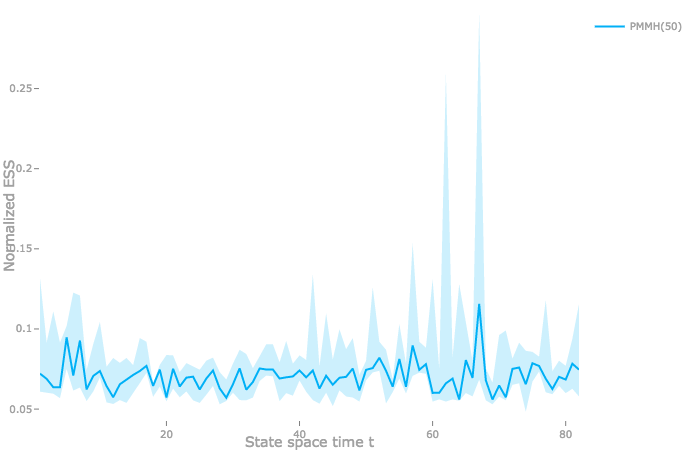
\includegraphics[width=0.8\textwidth]{ESS_PMMH_3.png}
    \caption{Normalized \acrfull{ESS} for 50 samples generated via the PMMH algorithm with 50 particles. The \gls{ESS}s are averaged on 8 runs.}
    \label{fig:ESS_PMMH}
\end{figure}


\subsection{\acrlong{PGAS}}
To our knowledge, the first article to tackle the path degeneracy problem is the \gls{PGAS} paper \cite{Lindsten:2014uw} (described in Subsection \ref{PMCMC}).
Yet, Van de Meent et al \cite{vandeMeent:2015uk} who proposed an adapted version for \glspl{PPL}, wrote ``Implementing PGAS in the context of probabilistic programs poses technical challenges when programs can make use of recursion and memoization''. \gls{PGAS} is therefore non-trivial to implement so that it can handle the type of models we are interested in, which make use of memoization.

\subsection{\acrlong{IPMCMC}}
Hopefully, Rainforth et al \cite{Rainforth:2016wq} developed another algorithm to alleviate the path degeneracy issue.
In \gls{IPMCMC}, a pool of \gls{CSMC} and unconditional \gls{SMC} algorithms are ran as parallel processes, referred as nodes. After each run of this pool, successive Gibbs updates to the indexes of the \gls{CSMC} nodes are applied, such that the indices of the \gls{CSMC} nodes changes. Hence, the nodes from which retained particles are sampled can change from one MCMC iteration to the next. This lets trading off exploration (\gls{SMC}) and exploitation (\gls{CSMC}) to achieve improved mixing of the Markov chains. Crucially, the pool provides numerous candidate indices at each Gibbs update, giving a significantly higher probability that an entirely new retained particle will be “switched in” than in non-interacting alternatives.

Another of our contribution is the implementation of this \gls{IPMCMC} algorithm in Turing. The implementation does not yet make use of parallelization, but sequentially samples from \gls{CSMC} and \gls{SMC} nodes, by making use of existing implementations of these two algorithms.
The code can be found online \footnote{see \url{https://github.com/emilemathieu/Turing.jl/blob/feature-334/src/samplers/ipmcmc.jl}}, it is currently reviews as a pull request so as to be merged in the official repository \footnote{\url{https://github.com/yebai/Turing.jl/pull/351}}.
In the Gibbs sampling step of the new indices of the \gls{CSMC} nodes, we have to sample from a categorical distribution but we only have the log-weights for numerical stability reasons. We therefore make use of a smart trick \footnote{\url{https://stats.stackexchange.com/questions/64081/how-do-i-sample-from-a-discrete-categorical-distribution-in-log-space}} using Gumbels distributions to sample from this categorical distribution and staying in the log-space.

We ran a similar experiment than for the previous samplers. We chose a \gls{IPMCMC} sampler with 15 particles, 2 \gls{CSMC} nodes and 2 \gls{SMC} nodes. We reduced the number of particles compared to our experiment with \gls{PG} and \gls{PMMH}, so that the computational time be approximately similar. 
Figure \ref{fig:ESS_IPMCMC} shows the average (also 1st and 3rd) \gls{ESS} of the posterior samples for each $x_t$. Even if the results are a bit noisy, we can experientially see the improvement in sample quality compared to \gls{PG} and \gls{PMMH}.
The \gls{ESS} is relatively stable across all $t$ and vary around $0.42$. Moreover, Figure \ref{fig:IPMCMCxscatter} shows posterior samples for $x_1$ and $x_{82}$ generated by \gls{IPMCMC}, similarly to Figure \ref{fig:posterior_samples_time} for \gls{PG}. We can see that neither samples of $x_1$ and $x_{82}$ are sticky, especially compared with samples from \gls{PG}. Figure \ref{fig:IPMCMC_x_hist} shows the corresponding histograms. Furthermore, Figure \ref{fig:IPMCMC_S_MLEFIT} shows posterior samples of $\frac{1}{\theta}$, along with a gamma distribution whose parameters have been fitted by maximising likelihood.
We can conclude that the \gls{IPMCMC} algorithm is the most efficient sampler we have considered for our model. Moreover it could be improved by running the \gls{CSMC} and \gls{SMC} nodes in a parallel way.

\begin{figure}[h!]
\centering
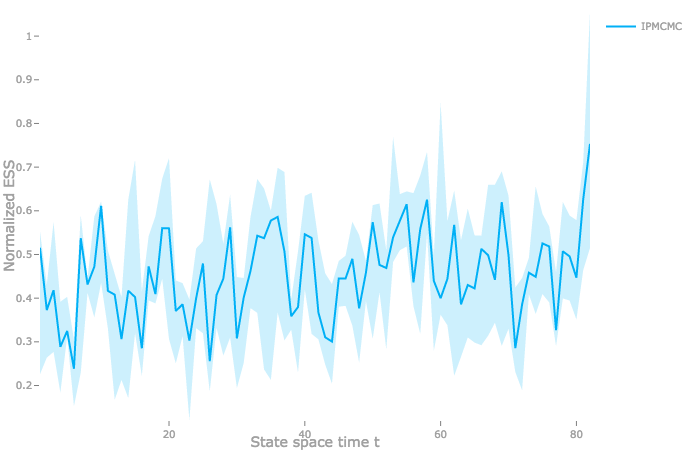
\includegraphics[width=0.8\textwidth]{ESS_IPMCMC_1.png}
    \caption{Normalized \acrfull{ESS} for 50 samples generated via the IPMCMC algorithm with 15 particles, 2 CSMS nodes and 2 SMC nodes. The \gls{ESS}s are averaged on 8 runs.}
    \label{fig:ESS_IPMCMC}
\end{figure}

\begin{figure}[h!]
  \centering
  \begin{minipage}[b]{0.48\textwidth}
    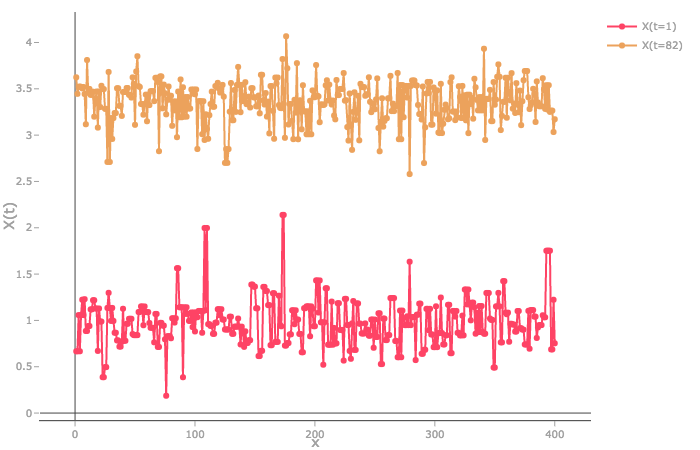
\includegraphics[width=\textwidth]{IPMCMC_X_scatter.png}
    \caption{Samples from the \gls{IPMCMC} sampler of the first $x_1$ and the last $x_{82}$ mixture components.}
    \label{fig:IPMCMCxscatter}
  \end{minipage}
  \hfill
  \begin{minipage}[b]{0.48\textwidth}
    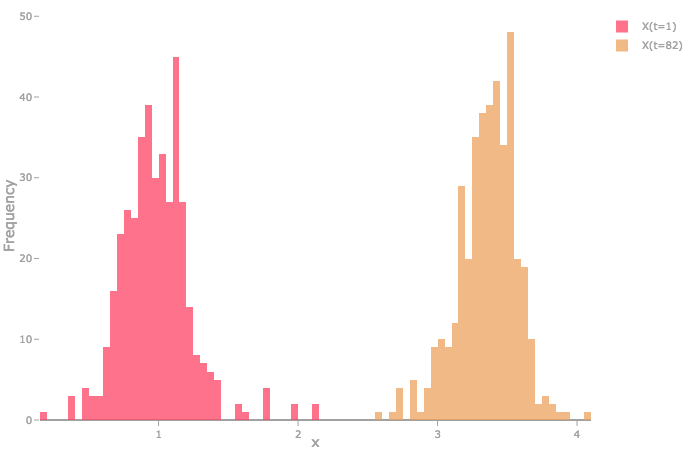
\includegraphics[width=\textwidth]{IPMCMC_X_hist.png}
    \caption{Histograms of posterior samples of $x_1$ and $x_{82}$ generated by an \gls{IPMCMC} sampler.}
    \label{fig:IPMCMC_x_hist}
  \end{minipage}
\end{figure}

\begin{figure}[h!]
\centering
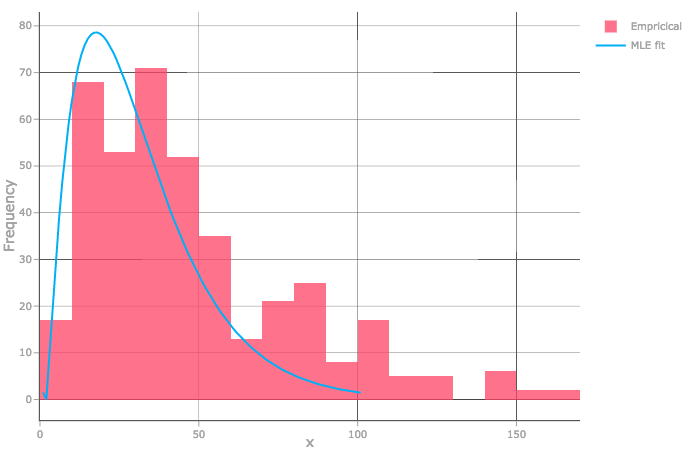
\includegraphics[width=0.8\textwidth]{IPMCMC_S_MLEFIT.png}
    \caption{Histogram of posterior samples of $\frac{1}{\theta}$, along with a Gamma distribution fitted by maximisation of the likelihood.}
    \label{fig:IPMCMC_S_MLEFIT}
\end{figure}

The current \gls{IPMCMC} algorithm \cite{Rainforth:2016wq} does not allow the explicit sampling of the global parameters; similarly to the \acrlong{CSMC} algorithm. It only targets $ p(x_{1:T}|y_{1:T}) \propto p(x_{1:T},y_{1:T})$, with the global parameters $\theta$ being implicitly included in the states variables $x_{1:T}$ (specifically with $x_1$ in our case). I have therefore designed an extended version of this algorithm -- and am currently working on the proof -- which explicitly targets $p(\theta, x_{1:T}|y_{1:T})$. The implementation I have already implemented this new algorithm in Turing so that I can easily compare it to other existing algorithms such as \gls{PG} and \gls{IPMCMC}, and in the hope to be merged in the official repository of Turing.
This work is likely to be submitted as a workshop paper. The main idea is to alternate sampling $x^{j}_{1:T} \sim p_\theta^{j}(\cdot|x^j_{1:T},y_{1:T})$ for the \gls{CSMC} nodes and $x^{j}_{1:T} \sim p_\theta^{\text{SMC}}(\cdot|y_{1:T})$ for \gls{SMC} nodes, with global parameter Gibbs steps $\theta^j \sim p(\cdot|x^j_{1:T},y_{1:T})$ for \gls{CSMC} nodes, but a unique step $\theta^{\text{SMC}} \sim p(\cdot|x^\text{SMC}_{1:T},y_{1:T})$ (with $x^\text{SMC}_{1:T}$ being randomly chosen between \gls{CSMC}'s $\{x^j_{1:T}\}_{j=1,\dots,P}$).
Listing \ref{code:IPMCMC} below shows how the constructor of this \gls{IPMCMC}'s extension is called with our implementation.

\begin{lstlisting}[caption={Extension of IPMCMC sampler constructor written in Turing.jl.},captionpos=b,label=code:IPMCMC]
N_CSMC = 2
N_nodes = 2 * N_CSMC
N_samples = 50 / N_CSMC
N_particles = 50
sampler = IPMCMC(N_particles, N_samples, N_nodes, N_CSMC, HMC(1,0.2,3,:$\theta$), :x)
\end{lstlisting}

We also ran experimentations on the extended version of \gls{IPMCMC}, by using an \gls{HMC} update for the global parameter $\theta$ (with 3 leapfrog steps of size 0.2). The mixing results are shown in Figure \ref{fig:ESS_MIPMCMC}, unfortunately it is unclear that the mixing of posterior samples is improved compared to the usual \gls{IPMCMC}. Further experimentations are needed, especially with more samples and more runs for averaging, since the noise of the experimentations is unfortunately quite high. It would also be interesting to compare algorithms by minimum \gls{ESS} (across all $t$), divided by computation time. Indeed, the user is interested to have high quality sample for all $t$, in a minimum time. It would also be interesting to compare these metrics with samples generated by model-specific samplers, such as the ones described in Section \ref{BNP_MCMC}.

\begin{figure}[h!]
\centering
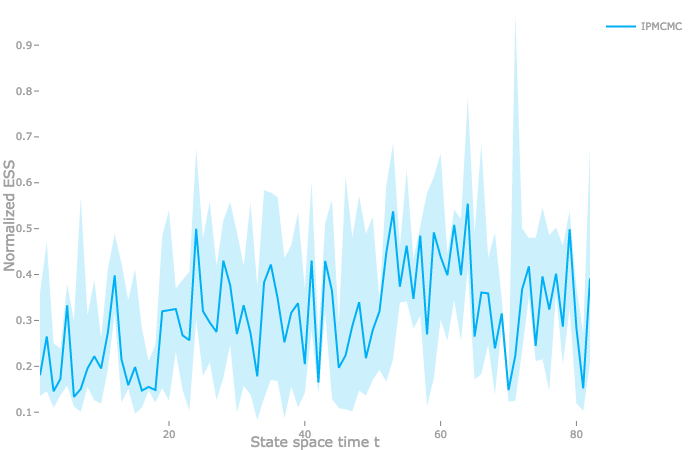
\includegraphics[width=0.8\textwidth]{ESS_MIPMCMC_1.png}
    \caption{Normalized \acrfull{ESS} for 50 samples generated via the extended version of IPMCMC algorithm with 15 particles, 2 CSMS nodes and 2 SMC nodes. The \gls{ESS}s are averaged on 8 runs.}
    \label{fig:ESS_MIPMCMC}
\end{figure}

\section{Open questions}
In this section we introduce related open questions on which we are currently working on.

% \paragraph{State representation}
% We casted this mixture model as a state-space model, but it is not completely clear how should the state be represented from an efficiency perspective. The state at time $t$ could be $(\{X_j^\star\}_{j=1}^k, \{z_i\}_{i=1}^t)$  where $k$ is the number of different component until now, $\{X_j^\star\}_{j=1}^k$ the (unique) mixture components, and $\{z_i\}_{i=1}^N$ the individual assignments. Yet it could also simply be $\{X_i\}_{i=1}^t$.
% Should we also explicitly represent the sticks lengths $\{{Z}_j\}_{j=1}^k$ in the \gls{PPL} model ?

\paragraph{Models}
For now we focused on infinite mixture models but our approach may be easily extended to other \gls{BNP} models, such as the infinite \acrlong{HMM} \cite{Beal02theinfinite} or latent feature models \cite{Ghahramani:2006tp} since a stick-breaking process for the \acrlong{IBP} has been developed \cite{stick-breaking-ibp}.

\paragraph{Posterior sampler}
For now we worked on existing samplers (\gls{SMC}, \gls{PG}, \gls{PMMH}, \gls{PGAS} and \gls{IPMCMC}), but we are thinking about developing (or extending) a sampler tailored for a specific model. A generic proposal, different (and hopefully better) than the prior might be developed.
Moreover, an interesting idea from Del Moral \& Murray \cite{DelMoral:2015jk} extending \gls{SMC} could be used. They introduce a schedule of intermediate weighting and resampling times between observation times, which guide particles towards the final state.
